\documentclass[12pt, a4paper, oneside]{article}
\usepackage{amsmath, amsthm, amssymb, bm, graphicx, hyperref, mathrsfs}
\usepackage{geometry}
\usepackage{amsmath}
\newtheorem{theorem}{Theorem}
\newtheorem{lemma}{Lemma}
\usepackage{hyperref}
\usepackage{mathrsfs}
\usepackage[ruled, lined, linesnumbered, commentsnumbered, longend]{algorithm2e}
\usepackage{booktabs}
\usepackage{breqn}
\usepackage{natbib}
\usepackage{amsmath}
\numberwithin{equation}{section}
\usepackage[ruled,linesnumbered]{algorithm2e}
\usepackage[UTF8]{ctex}
\usepackage{subfigure}

\title{\textbf{Hierarchical Heterogeneous Analysis of High-Dimensional Data}}
\author{Yan Ren \\ 2021103739}
\date{\today}
\linespread{1.5}
\newcounter{problemname}
\newenvironment{problem}{\stepcounter{problemname}\par\noindent\textsc{Problem \arabic{problemname}. }}{\\\par}
\newenvironment{solution}{\par\noindent\textsc{Solution. }}{\\\par}
\newenvironment{note}{\par\noindent\textsc{Note of Problem \arabic{problemname}. }}{\\\par}
\newcommand{\nysm}{Nystr$\ddot{\rm o}$m Method}
\geometry{a4paper, scale = 0.8}

\begin{document}
	
\maketitle
\newpage
\tableofcontents
\newpage

\section{Model}

\begin{itemize}
	\item $X = (X_1,...,X_n)^{T} \in \mathbb{R}^{n\times p}$, type \uppercase\expandafter{\romannumeral1} features (main G) for all observations, where $X_i \in \mathbb{R}^{p}$;
	\item $Z = (Z_1,...,Z_n)^{T} \in \mathbb{R}^{n\times q}$, type \uppercase\expandafter{\romannumeral2} features (main E) for all observations, where $Z_i \in \mathbb{R}^{q}$;
	\item $y = (y_1,...,y_n)^{T} \in \mathbb{R}^{n}$, the response vector.
\end{itemize}

\subsection{Basic Model}

简化后的异质性模型为:

\begin{equation}
	y_i = X_i^T \beta_i^\prime + Z_i^T\alpha_i^\prime + \epsilon_i
	\label{eq:model}
\end{equation}

其中 $\epsilon_i \sim (iid) N(0, \sigma^2)$

假设所有观测大组可根据基因(X)进行划分,大组中根据环境/图片特征变量(Z)进行进一步的划分。假设有 $K$ 个亚组,则相同亚组中的样有相同参数。

\subsection{Object Function}

基于高斯混合分布,重参数化后最小化目标函数为(负对数似然+惩罚):

\begin{equation}
	\begin{aligned}
		\mathcal{L}(\beta,\alpha, \pi | X, y) &= -\frac1n\sum_{i=1}^{n}\log{p_Y(y)} + \operatorname{pen}(\beta^\prime, \alpha^\prime)\\
		&= -\frac1n\sum_{i=1}^{n}\log{(\sum_{k=1}^{K}\pi_k f_k(y_i|X_i, Z_i))} + \operatorname{pen}(\beta^\prime, \alpha^\prime)\\
		&= -\frac1n\sum_{i=1}^{n}\log\left\lbrace \sum_{k=1}^{K}\pi_k \frac{1}{\sqrt{2\pi}\sigma_k} \exp\left(   -\frac{1}{2\sigma_k^2}   \left(y_i - X_i^T \beta^\prime_k - Z_i^T \alpha^\prime_k \right)^2      \right)  \right\rbrace + \operatorname{pen}(\beta^\prime, \alpha^\prime)\\
		&= -\frac1n\sum_{i=1}^{n}\log\left\lbrace \sum_{k=1}^{K}\pi_k \frac{\rho_k}{\sqrt{2\pi}} \exp\left(   -\frac{1}{2}   \left(y_i\rho_k - X_i^T \beta_k - Z_i^T \alpha_k \right)^2      \right)  \right\rbrace  + \operatorname{pen}(\beta, \alpha)\\
	\end{aligned}
	\label{eq:object}
\end{equation}

其中重参数化为 $\beta_k = \beta_k^\prime / \sigma_k, \rho_k = 1/\sigma_k$,惩罚函数为

\begin{equation}
	\begin{aligned}
		\operatorname{pen}(\beta, \alpha)
		&=\sum_{k=1}^{K}\sum_{j=1}^{p} \operatorname{pen}\left(|\beta_{kj}|, \lambda_{1}\right) + \sum_{k=1}^{K}\sum_{s=1}^{q} \operatorname{pen}\left(|\alpha_{ks}|, \lambda_{1}\right)\\
		&+\sum_{k<k^{\prime}} \operatorname{pen}\left(\sqrt{\left\|\beta_{k}-\beta_{k^{\prime}}\right\|_{2}^{2}+\left\|\alpha_{k}-\alpha_{k^{\prime}}\right\|_{2}^{2}}, \lambda_{2}\right) \\
		&+\sum_{k<k^{\prime}} \operatorname{pen}\left(\left\|\beta_{k}-\beta_{k^{\prime}}\right\|_{2}, \lambda_{3}\right)
	\end{aligned}
	\label{eq:penalty}
\end{equation}

第一项惩罚保证基因相关系数的稀疏性;第二,第三项惩罚共同作用以致模型呈现层级结构(Hierarchy).

\subsection{Penalty Function}

MCP 惩罚函数

\begin{equation}
	\label{eq:mcp}
	pen_{(\lambda, a)}(\beta) = \left\{
	\begin{aligned}
		&\lambda |\beta| - \frac{\beta^2}{2a}, & |\beta| \leq a\lambda \\
		&\frac{a}{2}\lambda^2, & |\beta| > a\lambda
	\end{aligned}
	\right.
\end{equation}

MCP 惩罚函数对参数求偏导得

\begin{equation}
	pen_{(\lambda, a)}^{\prime}(\beta)= \begin{cases}\operatorname{sgn}(\beta)\left(\lambda-\frac{|\beta|}{a}\right) & |\beta| \leq a \lambda \\ 0 & \text { otherwise }\end{cases}
\end{equation}

超参数 a 常取为大于 1 的数。

\section{Computation}

\subsection{Transformation}

采用 EM 算法。E 步更新 $\pi$,M 步更新参数 $\beta, \alpha$。引入变量 $C_i$ 用于指示每个样本属于哪个类别,有后验概率如 \ref{eq:posterier} 所示

\begin{equation}
	q_{C_i}(c_i) = \frac{{\pi_{c_i} f_{c_i}(y_i|X_i,Z_i)}}{\displaystyle\sum_{k=1}^{K}\pi_{k} f_{k}(y_i|X_i,Z_i)}
	\label{eq:posterier}
\end{equation}

目标函数 \ref{eq:object} 中对数似然部分可以放缩如下
\begin{equation}
	\begin{aligned}
		\log p_Y (y)  &= log \sum_{k = 1}^{K}p_{Y,C}(y,c) \\
		&= log E_{q_C}\left(\frac{p_{Y,C}(y,c)}{q_C(c)}\right) \\
		&\geq E_{q_C}\left(\frac{p_{Y,C}(y,c)}{q_C(c)}\right) \\
		&= E_{q_C} \left(log p_{Y,C}(y,c)\right) - E_{q_C}\left(log q_C(c)\right)
	\end{aligned} 
\label{eq:logtrans}
\end{equation}

综上,目标函数可以放缩(根据 Gaussian mixture models and the EM algorithm)为 

\begin{equation}
	\begin{aligned}
		\mathcal{L}(\beta,\alpha, \pi | X, y)
		&= -\sum_{i=1}^{n}\log{p_Y(y)} + \operatorname{pen}(\beta, \alpha)\\
		&\leq -E_{q_C} \left(log p_{Y,C}(y,c)\right) + E_{q_C}\left(log q_C(c)\right)+ \operatorname{pen}(\beta, \alpha)\\
	\end{aligned}
\label{eq:object2}
\end{equation}

在 M 步更新参数 $\beta, \alpha$ 式 \ref{eq:object2} 中 $E_{q_C}(log q_C(c))$ 与参数无关。而 $E_{q_C} \left(log p_{Y,C}(y,c)\right)$ 可以进一步变形

\begin{equation}
	\begin{aligned}
		E_{q_C}log p_{Y,C}(y,c) &= E_{q_C} log \left(p_C(c) p_{Y|C}(y)\right)\\
		&= E_{q_C} log \left(\prod^{n}_{i=1} p_{C_i}(c_i) p_{Y_i|C_i}(y_i) \right) \\
		&= E_{q_C} log \left(\prod^{n}_{i=1}\prod^{K}_{k=1} \pi_{c_i} f_{Y_i|C_i}(y_i) \right)^{I(C_i=k)} \\
		&= E_{q_C} \sum^{n}_{i=1}\sum^{K}_{k=1} I(C_i=k)\left( log\pi_{c_i} + log f_{Y_i|C_i}(y_i) \right) \\
		&= \sum^{n}_{i=1}\sum^{K}_{k=1} E_{q_C} I(C_i=k)\left( log\pi_{c_i} + log f_{Y_i|C_i}(y_i) \right) \\
		&= \sum^{n}_{i=1}\sum^{K}_{k=1} q_{C_i}(k)\left( log\pi_{c_i} + log f_{Y_i|C_i}(y_i) \right) \\
		&= \sum^{n}_{i=1}\sum^{K}_{k=1} q_{C_i}(k)\left(log\pi_{c_i} +log\rho_k - \frac{1}{2}log 2\pi - \frac{1}{2}(y_i\rho_k - X_i^T \beta_k - Z_i^T \alpha_k)^2\right) \\
		&= \sum_{i=1}^{n}\sum^{K}_{k=1} q_{C_i}(k)\left(C-\frac{1}{2}(y_i\rho_k - X_i^T \beta_k - Z_i^T \alpha_k)^2 \right)
	\end{aligned}
\end{equation}

其中 $C$ 为与更新参数无关的常数项。此时最小化目标为原目标函数的上界,表达式为

\begin{equation}
	\begin{aligned}
		\mathcal{L}(\beta,\alpha|\pi, X, y)
		=& -\frac1n\sum_{i=1}^{n}\log{p_Y(y)} + \operatorname{pen}(\beta, \alpha)\\
		\leq& -\frac1nE_{q_C} \left(log p_{Y,C}(y,c)\right) + \operatorname{pen}(\beta, \alpha) \\
		=& -\frac1n\sum_{i=1}^{n}\sum^{K}_{k=1} q_{C_i}(k)\left(C-\frac{1}{2}(y_i\rho_k - X_i^T \beta_k - Z_i^T \alpha_k)^2 \right) \\
		&+ \sum_{k=1}^{K} \operatorname{pen}\left(\Vert\beta_{k}\Vert_2, \lambda_{1}\right) 
		+ \sum_{k=1}^{K} \operatorname{pen}\left(\Vert\alpha_{k}\Vert_2, \lambda_{1}\right) \\
		&+\sum_{k<k^{\prime}} \operatorname{pen}\left(\sqrt{\left\|\beta_{k}-\beta_{k^{\prime}}\right\|_{2}^{2}+\left\|\alpha_{k}-\alpha_{k^{\prime}}\right\|_{2}^{2}}, \lambda_{2}\right) \\
		&+\sum_{k<k^{\prime}} \operatorname{pen}\left(\left\|\beta_{k}-\beta_{k^{\prime}}\right\|_{2}, \lambda_{3}\right) \\
	\end{aligned}
	\label{eq:object_coef_related}
\end{equation}

\subsection{MCP}

$\beta$, $z$ 均为 $p$ 维向量,现假设目标函数有
\begin{equation}
	\mathcal{L}(x;\lambda) = \frac{\rho}{2}\Vert x - z\Vert_2^2 + \operatorname{pen}(\Vert x\Vert_2;\lambda)
\end{equation}
则 $x$ 对应解为
\begin{equation}
	x = \begin{cases}\frac{S\left(z, \frac{\lambda}{\rho}\right)}{1-\frac{1}{a \rho}} & \text { if }|z| \leq a \lambda \\ z & \text { if }|z|>a \lambda\end{cases}
\end{equation}

其中 $S(.,.)$ 为 soft thresholding operator,定义如下
\begin{equation}
	S(x, t)=\operatorname{sign}(x)(|x|-t)_{+}=x\left(1-\frac{t}{|x|}\right)_{+}
\end{equation}

故 $x$ 解也可写为
\begin{equation}
	x = \begin{cases}\frac{
	z\left(1 - \frac{\lambda}{|z|\rho}\right)_+
}{1-\frac{1}{a \rho}} & \text { if }|z| \leq a \lambda \\ z & \text { if }|z|>a \lambda\end{cases}
\end{equation}


\section{Model Preparation}

\subsection{Version 1 - P for $\beta$ ADMM}

为了尝试推导以及检验代码正确性,先尝试构建较为简单的模型进行实验。考虑以下目标函数
\begin{equation}
\begin{aligned}
	\mathcal{L}^{(1)}(\beta,\alpha) &= -\frac1n\sum_{i=1}^{n}\sum^{K}_{k=1} q_{C_i}(k)\left(C-\frac{1}{2}(y_i\rho_k - X_i^T \beta_k - Z_i^T \alpha_k)^2 \right) + \sum_{k=1}^{K}\sum_{j=1}^{p} \operatorname{pen}\left(|\beta_{kj}|, \lambda_{1}\right) \\
	&= \frac{1}{2n}\sum_{i=1}^{n}\sum^{K}_{k=1} q_{C_i}(k)\left(y_i\rho_k - X_i^T \beta_k - Z_i^T \alpha_k \right)^2 + \sum_{k=1}^{K}\sum_{j=1}^{p} \operatorname{pen}\left(|\beta_{kj}|, \lambda_{1}\right) + C \\
\end{aligned}
\end{equation}

C 表示与更新参数无关的项,后面均省略。对于类别 $k$ 目标函数为

\begin{equation}
	\begin{aligned}
		\mathcal{L}_k^{(1)}(\beta_k,\alpha_k)=\frac{1}{2n}\sum_{i=1}^{n} q_{C_i}(k)\left(y_i\rho_k - X_i^T \beta_k - Z_i^T \alpha_k \right)^2 + \sum_{j=1}^{p} \operatorname{pen}\left(|\beta_{kj}|, \lambda_{1}\right)
	\end{aligned}
\end{equation}

对应增广拉格朗日函数为

\begin{equation}
	\begin{aligned}
		\mathcal{L}_{k,\rho}^{(1)}(\beta_k,\alpha_k,\tau) &=\frac{1}{2n}\sum_{i=1}^{n} q_{C_i}(k)\left(y_i\rho_k - X_i^T \beta_k - Z_i^T \alpha_k \right)^2 + \sum_{j=1}^{p} \operatorname{pen}\left(|\beta_{kj}|, \lambda_{1}\right) \\
		& + \sum_{j=1}^{p}\operatorname{pen}\left(|\theta_{kj}|, \lambda_{1}\right)
		+ \tau^T (\beta_k - \theta_k) + \frac{\rho}{2}\Vert\beta_k - \theta_k\Vert_2^2
	\end{aligned}
\label{eq:auglagrange_k}
\end{equation}

$\tau$ 为对应的拉格朗日乘子(向量),$\rho>0$ 为拉格朗日参数。给定 $(\beta_k^{(t)},\alpha_k^{(t)},\tau^{(t)})$ 则第 $t+1$ 步更新写为

\begin{align}
	&{\beta}_k^{(t+1)} \in \underset{{\beta} \in \mathbb{R}^p}{\arg \min }\  \mathcal{L}_{k,\rho}^{(1)}\left({\beta}, {\theta}^{(t)}, {\tau}^{(t)}\right) \\
	&{\theta}_k^{(t+1)} \in \underset{{\theta} \in \mathbb{R}^p}{\arg \min }\  \mathcal{L}_{k,\rho}^{(1)}\left({\beta}^{(t+1)}, {\theta}, {\tau}^{(t)}\right) \\ 
	&{\tau}^{(t+1)}={\tau}^{(t)}+\rho\left({\beta}^{(t+1)}-{\theta}^{(t+1)}\right) 
\end{align}

\paragraph{Update $\beta_k$}

式 \ref{eq:auglagrange_k} 中与 $\beta_k$ 相关的项为

\begin{equation}
	\begin{aligned}
		\mathcal{L}_{k,\rho}^{(1)}(\beta_k) &=\frac{1}{2n}\sum_{i=1}^{n} q_{C_i}(k)\left(y_i\rho_k - X_i^T \beta_k - Z_i^T \alpha_k \right)^2 + \sum_{j=1}^{p} \operatorname{pen}\left(|\beta_{kj}|, \lambda_{1}\right) \\
		& + \tau^T (\beta_k - \theta_k) + \frac{\rho}{2}\Vert\beta_k - \theta_k\Vert_2^2
	\end{aligned}
\end{equation}

对 $\beta_k$ 求偏导,得

\begin{equation}
	\beta_k = \left(n^{-1}X^TW_k X+\rho I_p \right)^{-1}\left(n^{-1}X^T W^\prime_k y^{\beta_k}+\rho \theta_k-\tau\right)
\end{equation}

其中 $y^{(\beta_k)} = y\rho_k - Z\alpha_k$,$ W_k = \rho_k diag(q_{C_1}(k),...,q_{C_n}(k))$,$I_p$ 为 $p$ 维单位矩阵。

\paragraph{Update $\theta_k$}

式 \ref{eq:auglagrange_k} 中与 $\theta_k$ 相关的项为

\begin{equation}
	\begin{aligned}
		\mathcal{L}_{k,\rho}^{(1)}(\beta_k) &= \sum_{j=1}^{p}\operatorname{pen}\left(\theta_{kj}, \lambda_{1}\right) + \tau^T (\beta_k - \theta_k) + \frac{\rho}{2}\Vert\beta_k - \theta_k\Vert_2^2 \\
		&= \frac{\rho}{2}\Vert\theta_k - z_k\Vert_2^2 +  \sum_{j=1}^{p}\operatorname{pen}\left(\theta_{kj}, \lambda_{1}\right)
	\end{aligned}
\end{equation}
其中 $z_k = \beta_k + \frac{\tau}{\rho}$.

故 $\theta_k = (\theta_{k1},...,\theta_{kp})$ 的解为
\begin{equation}
	\theta_{kj} = \begin{cases}\frac{S\left(z_{kj}, \frac{\lambda}{\rho}\right)}{1-\frac{1}{a \rho}} & \text { if }|z_{kj}| \leq a \lambda \\ z_{kj} & \text { if }|z_{kj}|>a \lambda\end{cases}
\end{equation}

\paragraph{Update $\rho_k$}

惩罚项不涉及 $\rho_k$,更新 $\rho_k$ 只需要考虑拟合项。式 \ref{eq:auglagrange_k} 中未完全表示出 $\rho_k$ 相关的项,原待最小化的目标函数中与 $\rho_k$ 有关的项应为 \ref{eq:rho-k-update-v1}.(注意此处 $\rho$ 表示拉格朗日参数,$rho_k = 1/\sigma_k$ 为高斯分布中的参数)

\begin{equation}
	\begin{aligned}
		\mathcal{L}_{k,\rho}^{(1)}(\rho_k) &= 
		-\frac1n \sum_{i=1}^{n} q_{C_i}(k)\left(log \rho_k - \frac12 (y_i\rho_k - X_i^T\beta_k - Z_i^T\alpha_k)^2\right)
	\end{aligned}
\label{eq:rho-k-update-v1}
\end{equation}

对 $\rho_k$ 求导得

\begin{equation}
	\begin{aligned}
		\frac{\partial\mathcal{L}_{k,\rho}^{(1)}(\rho_k)}{\partial \rho_k} &= 
		-\frac1n \sum_{i=1}^{n} q_{C_i}(k)\left(1/\rho_k - (y_i\rho_k - X_i^T\beta_k - Z_i^T\alpha_k)y_i\right)
	\end{aligned}
\end{equation}

$\frac{\partial\mathcal{L}_{k,\rho}^{(1)}(\rho_k)}{\partial \rho_k} = 0$ 时,有下式成立。

\begin{equation}
	\begin{aligned}
		\sum_{i=1}^{n}q_{C_i}(k)\left( -\rho_k^2 y_i^2 + \rho_k(X_i^T\beta_k + Z_i^T\alpha_k)y_i + 1 \right) &= 0 \\
		-y^TW_k y \rho_k^2 + (X\beta_k+Z\alpha_k)^T W_k y \rho_k + I_n^T W_k I_n &= 0\\
	\end{aligned}
	\label{eq:rho-k-update2-v1}
\end{equation}

这是一个一元二次方程求根问题,因为 $\rho_k$ 应为正值,取两个根中的正值,解为

\begin{equation}
	\rho_k = \frac{-B-\sqrt{B^2 - 4AC}}{2A}
\end{equation}

其中 $A = -y^TW_k y,\ B = (X\beta_k+Z\alpha_k)^T W_k y,\ C = 1_n^T W_k 1_n.$

若给定每个样本类别,等价于再各个类别内部使用 ADMM 方法进行迭代求解系数;若未知样本类别,使用 EM 算法进行估计,算法流程见 \ref{alg:simplest}

\IncMargin{1em} % 使得行号不向外突出 
\begin{algorithm}
	
	\SetKwInOut{Input}{Input}
	\SetKwInOut{Output}{Output} % 替换关键词
	
	\Input{数据 $y,X$,超参数 $n,p,K,a,\lambda,\rho$}
	\Output{$\beta_k,k=1,...,K$ 的估计值}
	\BlankLine
	
	初始化 $q_{C_i}(k) = \frac{1}{K}+\operatorname{N}(0,0.5^2), k=1,...,K,i=1,...,n$ 标准化; \\
	\Repeat
	{收敛($ \frac{\Vert\beta^{(iter)}-\beta^{(iter-1)}\Vert}{\Vert\beta^{(iter)}\Vert} $小于临界值)}
	{
		\For {$k\ in\ 1:K$}{
			$W_k = diag(q_{C_1}(k),...,q_{C_n}(k))$;\\
			更新 $\beta_k^{(iter)} = \left(n^{-1}X^TW_k X+\rho I_p \right)^{-1}\left(n^{-1}X^T W_k^\prime y^{\beta_k}+\rho \theta_k-\tau\right)$;\\
			更新 $\theta_k^{(iter)} = \begin{cases}\frac{S\left(z_k, \frac{\lambda}{\rho}\right)}{1-\frac{1}{a \rho}} & \text { if }\Vert z_k\Vert_2 \leq a \lambda \\ z & \text { if }\Vert z_k\Vert_2>a \lambda\end{cases}$; \\
			更新 $\tau^{(iter)} = \tau^{(iter-1)} + \rho (\beta_k^{(iter)}-\theta_k^{(iter)})$.\\
			更新 $\rho^{(iter)}_k = \frac{-B-\sqrt{B^2-4AC}}{2A}$.\\
			\qquad where $A = -y^TW_ky; B = (X\beta_k+Z\alpha_k)^TW_ky; C = 1_n^T W_k 1_n.$
		} 
		计算基于 $\beta_k^{(iter)}$ 得到的后验概率 $q_C$\\
		\qquad $q^{(iter)}_{C_i}(k) = \frac{{\pi_k^{(iter)} f_k(y_i;\beta_{k}^{(iter)}/\rho_k^{(iter)})}}{\sum_{{k^\prime}=1}^{K}\pi^{(iter)}_{k^\prime} f_{k^\prime}(y_i;\beta_{k\prime}^{(iter)}/\rho_k^{(iter)})}, k = 1,...,K$ \\
		更新 $\pi^{(iter)}_k = \frac{1}{n}\sum_{i=1}^{n}q^{(iter)}_{C_i}(k)$ \\
	}
	\caption{Version 1 with sparse penalty for $\beta$ (ADMM)}
	\label{alg:simplest}
\end{algorithm}
\DecMargin{1em}

实验结果大体如表 \ref{tb:res-v1} 所示。

\begin{table}[]
	\centering
	\begin{tabular}{ccccc}
		\toprule
		\textbf{p} & \textbf{非零个数} & \textbf{epsilon}            & \textbf{flexmix} & \textbf{自己迭代} \\
		\midrule
		8          & 3             & 0                           & 收敛到真值            & 收敛到真值         \\
		8          & 3             & $N(0,0.5^2)$ & 收敛到接近真值          & 收敛到接近真值       \\
		40         & 3             & 0                           & 全0估计             & 距离真值有差异,详情见表  \\
		40         & 3             & $N(0,0.5^2)$ & 全0估计             & 收敛到接近真值     \\
		\bottomrule 
	\end{tabular}
\label{tb:res-v1}
\end{table}

\subsection{Version 2 - P for $\beta$}

依旧对目标函数 
\begin{equation}
	\begin{aligned}
		\mathcal{L}^{(2)}(\beta,\alpha)=\frac{1}{2n}\sum_{i=1}^{n}\sum_{k=1}^{K} q_{C_i}(k)\left(y_i\rho_k - X_i^T \beta_k - Z_i^T \alpha_k \right)^2 + \sum_{k=1}^{K}\sum_{j=1}^{p} \operatorname{pen}\left(|\beta_{kj}|, \lambda_{1}\right) 
	\end{aligned}
\end{equation}

不同于上一节,现在直接对于 $\beta_{kj}$ 求偏导进行求解,而不用 ADMM 算法框架进行问题的转化。目标函数中与第 $k$ 类中的参数相关的部分写为 $\mathcal{L}^{(2)}_k$,见 \ref{eq:v2-object-k},其中 $y_{ik}^\prime = \rho_k y_i - X_{i(-j)}^T\beta_{k(-j)} - Z_i^T \alpha_k$,$y_k^\prime = (y_{1k}^\prime, ..., y_{nk}^\prime)^T \in \mathbb{R}^{n\times 1}$, $X_{i(-j)}$ 表示 $X_i$ 中除第 $j$ 列外的其他特征,$X_{(-j)} = (X_{1(-j)},...,X_{n(-j)})^T \in \mathbb{R}^{n\times(p-1)}$,$\tilde{X}_j = (X_{1j}, ..., X_{nj})^T \in \mathbb{R}^{n\times 1}$,$W_k = diag(q_{C_1}(k), ..., q_{C_n}(k)) \in \mathbb{R}^{n\times n}$

\begin{equation}
	\begin{aligned}
		\mathcal{L}^{(2)}_k (\beta_k, \alpha_k) &= \frac{1}{2n}\sum_{i=1}^{n} q_{C_i}(k)\left(y_i\rho_k - X_i^T \beta_k - Z_i^T \alpha_k \right)^2 + \sum_{j=1}^{p} \operatorname{pen}\left(|\beta_{kj}|, \lambda_{1}\right) \\
		&= \frac{1}{2n}\sum_{i=1}^{n} q_{C_i}(k)\left(y_{ik}^\prime - X_{ij} \beta_{kj} \right)^2 + \sum_{j=1}^{p} \operatorname{pen}\left(|\beta_{kj}|, \lambda_{1}\right) \\
		&=  \frac{1}{2n}\sum_{i=1}^{n} q_{C_i}(k)\left(y_{ik}^{\prime 2} - 2X_{ij} y_i^{\prime}\beta_{kj} + X_{ij}^2 \beta_{kj}^2\right) + \sum_{j=1}^{p} \operatorname{pen}\left(|\beta_{kj}|, \lambda_{1}\right) \\
		&= \frac{1}{2n}\left( \tilde{X_j}^T W_k \tilde{X_j} \beta_{kj}^2 - 2\tilde{X_j}^TW_k y_k^\prime \beta_{kj} + y_k^{\prime T}W_ky_k^\prime \right) + \sum_{j=1}^{p} \operatorname{pen}\left(|\beta_{kj}|, \lambda_{1}\right) \\
		&= \frac{\tilde{X_j}^T W_k \tilde{X_j}}{2n}\left( \beta_{kj}-\frac{\tilde{X_j}^TW_k y_k^\prime}{\tilde{X_j}^T W_k \tilde{X_j}} \right)^2 + \operatorname{pen}\left(|\beta_{kj}|, \lambda_{1}\right) + C
	\end{aligned}
\label{eq:v2-object-k}
\end{equation}

其中 C 与 $\beta_{kj}$ 无关,记 $u_{kj} = \tilde{X_j}^TW_k y_k^\prime$,$l_{kj} = \tilde{X_j}^T W_k \tilde{X_j}$,使得上式最小的 $\beta_{kj}$ 可表示为

\begin{equation}
	\beta_{kj} = 
	\begin{cases}
	\frac{S\left(\frac{u_{kj}}{l_{kj}}, \frac{n\lambda}{l_{kj}}\right)}{1-\frac{n}{al_{kj}}} = 
	\frac{S\left(u_{kj}, n\lambda\right)}{l_{kj}-\frac{n}{a}} & \text { if }|\frac{u_{kj}}{l_{kj}}| \leq a \lambda \\ 
	\frac{u_{kj}}{l_{kj}} & \text { if }|\frac{u_{kj}}{l_{kj}}|>a \lambda
\end{cases}
\end{equation}

算法流程如 \ref{alg:simplest-v2}

\IncMargin{1em} % 使得行号不向外突出 
\begin{algorithm}
	
	\SetKwInOut{Input}{Input}
	\SetKwInOut{Output}{Output} % 替换关键词
	
	\Input{数据 $y,X$,超参数 $n,p,K,a,\lambda,\rho$}
	\Output{$\beta_k,k=1,...,K$ 的估计值}
	\BlankLine
	
	初始化 $q_{C_i}(k) = \frac{1}{K}+\operatorname{N}(0,0.5^2), k=1,...,K,i=1,...,n$ 标准化,或用 flexmix 包结果初始化; \\
	\Repeat
	{收敛($ \frac{\Vert\beta^{(iter)}-\beta^{(iter-1)}\Vert}{\Vert\beta^{(iter)}\Vert} $小于临界值)}
	{
		\For {$k\ in\ 1:K$}{
			$W_k = diag(q_{C_1}(k),...,q_{C_n}(k))$;\\
			\For {$j\ in\ 1:p$}{
				$u_{kj} = (\rho_k y - X_{(-j)}\beta_{k(-j)} - Z\alpha_k)^T W_k \tilde{X_j}$\\
				$l_{kj} = \tilde{X_j}^T W_k \tilde{X_j}$ \\
			更新 $\beta_{k j}^{(iter)}= 
			\begin{cases}
				\frac{u_{k j}}{l_{k j}} & \frac{u_{k j}}{l_{kj}} > a \lambda \\
				\frac{S(\frac{u_{kj}}{l_{kj}}, n\lambda)}{1-\frac{n}{a}}, & \frac{u_{k j}}{L_{k j}} \leqslant a \lambda
			 \end{cases}$
			}
			更新 $\rho^{(iter)}_k = \frac{-B-\sqrt{B^2-4AC}}{2A}$.\\
			\qquad where $A = -y^TW_ky; B = (X\beta_k+Z\alpha_k)^TW_ky; C = 1_n^T W_k 1_n.$
		} 
		计算基于 $\beta_k^{(iter)}$ 得到的后验概率 $q_C$\\
		\qquad $q^{(iter)}_{C_i}(k) = \frac{{\pi_k^{(iter)} f_k(y_i;\beta_{k}^{(iter)}/\rho_k^{(iter)})}}{\sum_{{k^\prime}=1}^{K}\pi^{(iter)}_{k^\prime} f_{k^\prime}(y_i;\beta_{k\prime}^{(iter)}/\rho_k^{(iter)})}, k = 1,...,K$ \\
		更新 $\pi^{(iter)}_k = \frac{1}{n}\sum_{i=1}^{n}q^{(iter)}_{C_i}(k)$ \\
	}
	\caption{Version 2 with sparse penalty for $\beta$}
	\label{alg:simplest-v2}
\end{algorithm}
\DecMargin{1em}

实验中,若 n=400, p=8 $\beta_k$ 中非零项长度为 3(实验中设置 $\alpha_k = 0$,上面所有推导可忽略包含 $\alpha$ 项,同时包含 $\beta, \alpha$ 且不全为 0 的模型在第三部分实验),模型可以稳定收敛到真值,当增加误差项或者当 $p$ 增大时,会出现 3,-3 项估计准确而 1,-1 被压为零,或调整参数后出现部分零项估计非零,整个向量偏离真值的情况。在困难情况下使用 flexmix 包作为储值可以收敛。

\subsection{Version 3 - P for both $\beta,\alpha$}

此时目标函数表示为

\begin{equation}
	\begin{aligned}
		\mathcal{L}^{(3)}(\beta,\alpha)&=\frac{1}{2n}\sum_{i=1}^{n}\sum_{k=1}^{K} q_{C_i}(k)\left(y_i\rho_k - X_i^T \beta_k - Z_i^T \alpha_k \right)^2 \\
		&+ \sum_{k=1}^{K}\sum_{j=1}^{p} \operatorname{pen}\left(|\beta_{kj}|, \lambda_{1}\right) + \sum_{k=1}^{K}\sum_{s=1}^{q} \operatorname{pen}\left(|\alpha_{ks}|, \lambda_{1}\right) 
	\end{aligned}
\end{equation}

当 $\beta_k, \alpha_k$ 不全为 0 向量时,同时更新 $\beta_k$, $\alpha_k$ 的计算流程与上面两种情况相似,只需要注意当更新 $\beta_{kj}$ 时,对应 $y_i^\prime = \rho_k y_i - X_{i(-j)^T}\beta_{k(-j)} - Z_i^T\alpha_k$,$j=1,2,...,p$;而更新 $\alpha_{ks}$ 时,对应 $y_i^\prime = \rho_k y_i - Z_{i(-s)^T}\alpha_{k(-s)} - X_i^T\beta_k$,$s=1,2,...,q$;

在 $p, q$ 较大时更新难度增大,图 \ref{fig:compare-base} 对比了 $p=q=20$ 时全 0 初值及基于 flexmix 包结果继续迭代的参数距离真值距离随迭代次数变化曲线。

\begin{figure}
	\centering
	\subfigure[全 0 初值]{
		\begin{minipage}[t]{0.5\linewidth}
			\centering
			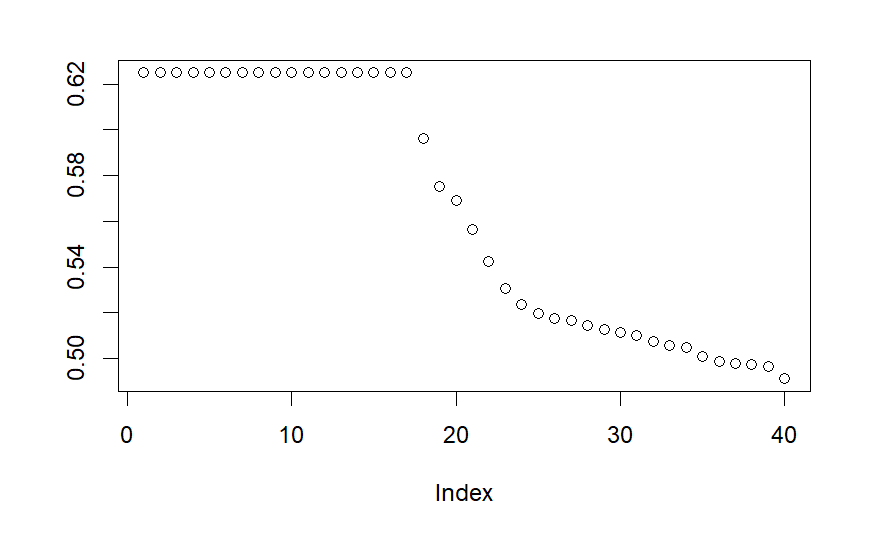
\includegraphics[width=3.5in]{img/v3_iter_base_0.png}
		\end{minipage}%
	}%
	\subfigure[flexmix 初值]{
		\begin{minipage}[t]{0.5\linewidth}
			\centering
			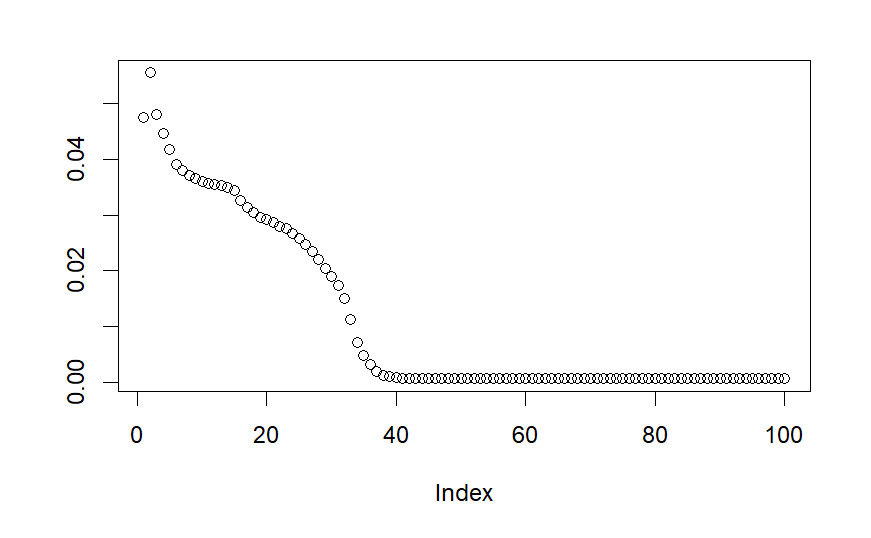
\includegraphics[width=3.5in]{img/v3_iter_base_flexmix.png}\\
		\end{minipage}%
	}%
	\caption{基于两种初值的参数收敛曲线(仅有 $\beta, \alpha$ 稀疏惩罚)}
	\label{fig:compare-base}
\end{figure}

已经验证,该框架下 $\alpha=0$ 时结果与 Version 2 完全相同。

\subsection{Version 4 - P for all}

该部分在 Version 3(仅有 $\beta, \alpha$ 的稀疏惩罚)基础上加上类别压缩惩罚函数,目标函数补全为最终的

\begin{equation}
	\begin{aligned}
		\mathcal{L}^{(4)}(\beta,\alpha)=&\frac{1}{2n}\sum_{i=1}^{n}\sum_{k=1}^{K} q_{C_i}(k)\left(y_i\rho_k - X_i^T \beta_k - Z_i^T \alpha_k \right)^2 \\
		&+ \sum_{k=1}^{K}\sum_{j=1}^{p} \operatorname{pen}\left(|\beta_{kj}|, \lambda_{1}\right) + \sum_{k=1}^{K}\sum_{s=1}^{q} \operatorname{pen}\left(|\alpha_{ks}|, \lambda_{1}\right)\\
		&+\sum_{k<k^{\prime}} \operatorname{pen}\left(\sqrt{\left\|\beta_{k}-\beta_{k^{\prime}}\right\|_{2}^{2}+\left\|\alpha_{k}-\alpha_{k^{\prime}}\right\|_{2}^{2}}, \lambda_{2}\right) \\
		&+\sum_{k<k^{\prime}} \operatorname{pen}\left(\left\|\beta_{k}-\beta_{k^{\prime}}\right\|_{2}, \lambda_{3}\right)
	\end{aligned}
\end{equation}

对应的增广拉格朗日函数为

\begin{equation}
	\begin{aligned}
		\mathcal{L}^{(4)}(\beta,\alpha,u,v,\xi,\zeta)=&\frac{1}{2n}\sum_{i=1}^{n}\sum_{k=1}^{K} q_{C_i}(k)\left(y_i\rho_k - X_i^T \beta_k - Z_i^T \alpha_k \right)^2 \\
		&+ \sum_{k=1}^{K}\sum_{j=1}^{p} \operatorname{pen}\left(|\beta_{kj}|, \lambda_{1}\right) + \sum_{k=1}^{K}\sum_{s=1}^{q} \operatorname{pen}\left(|\alpha_{ks}|, \lambda_{1}\right)\\
		&+ \sum_{k<k^{\prime}} \operatorname{pen}\left(\sqrt{\left\|v_{kk^\prime}\right\|_{2}^{2}+\left\|w_{kk^\prime}\right\|_{2}^{2}}, \lambda_{2}\right) \\
		&+ \sum_{k<k^{\prime}} \operatorname{pen}\left(\left\|v_{kk^\prime}\right\|_{2}, \lambda_{3}\right) \\
		&+ \sum_{k<k^{\prime}} \xi_{kk^{\prime}}^T(\beta_k - \beta_k^\prime - v_{kk^\prime}) + \frac{\tau}{2}\sum_{k<k^{\prime}}\Vert\beta_k - \beta_k^\prime - v_{kk^\prime}\Vert^2_2 \\
		&+ \sum_{k<k^{\prime}} \zeta_{kk^{\prime}}^T(\alpha_k - \alpha_k^\prime - w_{kk^\prime}) + \frac{\tau}{2}\sum_{k<k^{\prime}}\Vert\alpha_k - \alpha_k^\prime - w_{kk^\prime}\Vert^2_2
	\end{aligned}
\end{equation}

记 $H_1 = \varepsilon \otimes I_p \in \mathbb{R}^{\frac{K(K-1)}{2}p\times Kp}, H_2 = \varepsilon \otimes I_q \in \mathbb{R}^{\frac{K(K-1)}{2}q\times Kq}, \varepsilon = \{(e_k - e_{k^\prime}), k < {k^\prime}\}^T$. $e_k\in\mathbb{R}^{K\times 1}$ 为独热向量,除了第 $k$ 个元素为 1 外,其他元素都为 0;$I_p,I_q$ 分别表示维度为 $p\times p, q\times q$ 的单位对角阵。

另外,记

\begin{equation}
u_{k{k^\prime}} = (v^T_{kk^\prime}, w^T_{kk^\prime})^T
\end{equation}

则增广拉格朗日函数可以改写为

\begin{equation}
	\begin{aligned}
		\mathcal{L}^{(4)}(\beta,\alpha,u,v,\xi,\zeta)=&\frac{1}{2n}\sum_{i=1}^{n}\sum_{k=1}^{K} q_{C_i}(k)\left(y_i\rho_k - X_i^T \beta_k - Z_i^T \alpha_k \right)^2 \\
		&+ \sum_{k=1}^{K}\sum_{j=1}^{p} \operatorname{pen}\left(|\beta_{kj}|, \lambda_{1}\right) + \sum_{k=1}^{K}\sum_{s=1}^{q} \operatorname{pen}\left(|\alpha_{ks}|, \lambda_{1}\right)\\
		&+ \sum_{k<k^{\prime}} \operatorname{pen}\left(\Vert u_{kk^\prime}\Vert_2, \lambda_{2}\right) + \sum_{k<k^{\prime}} \operatorname{pen}\left(\left\|v_{kk^\prime}\right\|_{2}, \lambda_{3}\right) \\
		&+ \frac{\tau}{2}\Vert H_1 \beta - v + \frac{1}{\tau}\xi\Vert_2^2 + \frac{\tau}{2}\Vert H_2 \alpha - w + \frac{1}{\tau}\zeta\Vert_2^2
	\end{aligned}
\label{eq:v4-goal}
\end{equation}

注意维度 $\beta \in \mathbb{R}^{Kp\times 1}, \alpha \in \mathbb{R}^{Kq\times 1}, u, \xi \in \mathbb{R}^{\frac{K(K-1)p}{2}\times 1} , w, \zeta \in \mathbb{R}^{\frac{K(K-1)q}{2}\times 1}$。

\paragraph{Update $\beta_{kj}$}

式子 \ref{eq:v4-goal} 中与 $\beta_{kj}$ 相关的项写为

\begin{equation}
	\begin{aligned}
		\mathcal{L}^{(4)}(\beta_{kj})&=\frac{1}{2n}\sum_{i=1}^{n} q_{C_i}(k)\left(y_i\rho_k - X_i^T \beta_k - Z_i^T \alpha_k \right)^2 + \operatorname{pen}\left(|\beta_{kj}|, \lambda_{1}\right)+\frac{\tau}{2}\Vert H_1 \beta - v + \frac{1}{\tau}\xi\Vert_2^2 \\
		&= \frac{1}{2n}\left(l_{kj}\beta_{kj}^2 - u_{kj}\beta_{kj}\right) + \frac{\tau}{2}\left(l^\prime_{kj}\beta_{kj}^2 - u^\prime_{kj}\beta_{kj}\right) + \operatorname{pen}\left(|\beta_{kj}|, \lambda_{1}\right) + C(\beta_{kj}) \\
		&= \frac{1}{2}\left(L_{kj}\beta_{kj}^2 - U_{kj}\beta_{kj}\right) + \operatorname{pen}\left(|\beta_{kj}|, \lambda_{1}\right) + C(\beta_{kj}) \\
		&= \frac{L_{kj}}{2}\left(\beta_{kj}^2 - \frac{U_{kj}}{L_{kj}}\right)^2 + \operatorname{pen}\left(|\beta_{kj}|, \lambda_{1}\right) + C(\beta_{kj}) \\
	\end{aligned} 	
\end{equation}

其中 $C(\beta_{kj})$ 表示与 $\beta_{kj}$ 无关的项,记号补充说明如下:

\begin{equation}
	\left\{
	\begin{aligned}
		&l_{kj} = \tilde{X_j}^T W_k \tilde{X_j} \\
		&u_{kj} = \tilde{X_j}^T W_k \left(\rho_k y - X_{(-j)}\beta_{k(-j)} - Z\alpha_k\right) \\
		&l^\prime_{kj} = (H_1^T H_1)_{kj,kj} \\
		&u^\prime_{kj} = \left(H_1^T(v-\frac{1}{\tau}\xi)\right)_{kj} - \beta_{(-kj)}^T(H_1^T H_1)_{kj,(-kj)} \\
		&L_{kj} = \frac1n l_{kj} + \tau l^\prime_{kj} \\
		&U_{kj} = \frac1n u_{kj} + \tau u^\prime_{kj} \\
	\end{aligned}
	\right.
\end{equation}

$W_k = diag(q_{C_1}(k),...,q_{C_n}(k))$,解得

\begin{equation}
	\beta_{kj} = 
	\begin{cases}
		\frac{S\left(\frac{U_{kj}}{L_{kj}}, \frac{\lambda}{L_{kj}}\right)}{1-\frac{1}{aL_{kj}}} = 
		\frac{S\left(U_{kj}, \lambda\right)}{L_{kj}-\frac{1}{a}} & \text { if }|\frac{U_{kj}}{L_{kj}}| \leq a \lambda \\ 
		\frac{U_{kj}}{L_{kj}} & \text { if }|\frac{U_{kj}}{L_{kj}}|>a \lambda
	\end{cases}
\end{equation}

\paragraph{Update $\alpha_{ks}$}

更新过程完全类似 $\beta_{kj}$ 的更新。

\paragraph{Update $v_{kk^\prime},w_{kk^\prime}$}


式子 \ref{eq:v4-goal} 中与 $v_{kk^\prime},w_{kk^\prime}$ 相关的项写为

\begin{equation}
	\begin{aligned}
		\mathcal{L}^{(4)}(v_{kk^\prime},w_{kk^\prime})=&\sum_{k<k^{\prime}} \operatorname{pen}\left(\Vert u_{kk^\prime}\Vert_2, \lambda_{2}\right) + \sum_{k<k^{\prime}} \operatorname{pen}\left(\left\|v_{kk^\prime}\right\|_{2}, \lambda_{3}\right) \\
		&+ \frac{\tau}{2}\Vert H_1 \beta - v + \frac{1}{\tau}\xi\Vert_2^2 + \frac{\tau}{2}\Vert H_2 \alpha - w + \frac{1}{\tau}\zeta\Vert_2^2
	\end{aligned}
\end{equation}

记

\begin{equation}
	\left\{
	\begin{aligned}
		&\overline{v_{k{k^\prime}}} = \beta_k - \beta_{k^\prime} + \frac{1}{\tau}\xi_{k{k^\prime}}\\
		&\overline{w_{k{k^\prime}}} = \alpha_k - \alpha_{k^\prime} + \frac{1}{\tau}\zeta_{k{k^\prime}}\\
	\end{aligned}
	\right.
\end{equation}

\begin{equation}
	\left\{
	\begin{aligned}
		&u_{k{k^\prime}} = (v^T_{kk^\prime}, w^T_{kk^\prime})^T\\
		&\overline{u_{k{k^\prime}}} = (\overline{v_{kk^\prime}}^T, \overline{w_{kk^\prime}}^T)^T
	\end{aligned}
	\right.
\end{equation}

更新分为四种情况
\begin{enumerate}
	\item 若 $\Vert\overline{u_{kk^{\prime}}}\Vert_2 > a\lambda_2$ 且 $\Vert\overline{v_{kk^{\prime}}}\Vert_2 > a\lambda_3$,则 $w_{kk^{\prime}} = \overline{w_{kk^{\prime}}}$,$v_{kk^{\prime}} = \overline{v_{kk^{\prime}}}$;
	\item 若 $\Vert\overline{u_{kk^{\prime}}}\Vert_2 \leq a\lambda_2$ 且 $\displaystyle\frac{\left(1-\lambda_2/(\tau \Vert\overline u_{kk^{\prime}}\Vert_2 \Vert)\right)_+}{1-1/(a\tau)}\Vert\overline{v_{kk^{\prime}}}\Vert_2 > a\lambda_3$,\\ 则 $w_{kk^{\prime}} = \displaystyle\frac{\left(1-\lambda_2/(\tau \Vert\overline u_{kk^{\prime}}\Vert_2 \Vert)\right)_+}{1-1/(a\tau)}\overline{w_{kk^{\prime}}}$,$v_{kk^{\prime}} =\displaystyle\frac{\left(1-\lambda_2/(\tau \Vert\overline u_{kk^{\prime}}\Vert_2 \Vert)\right)_+}{1-1/(a\tau)} \overline{v_{kk^{\prime}}}$;
	\item 若 $\Vert\overline{w_{kk^{\prime}}}\Vert_2^2 + \left(\displaystyle\frac{\left(1-\lambda_3/(\tau \Vert\overline v_{kk^{\prime}}\Vert_2 \Vert)\right)_+}{1-1/(a\tau)}\right)^2 \Vert\overline{v_{kk^{\prime}}}\Vert_2^2 > (a\lambda_2)^2$ 且 $\Vert\overline{v_{kk^{\prime}}}\Vert_2 \leq a\lambda_3$,\\
	则 $w_{kk^{\prime}} = \overline{w_{kk^{\prime}}}$,$v_{kk^{\prime}} = \displaystyle\frac{\left(1-\lambda_3/(\tau \Vert\overline v_{kk^{\prime}}\Vert_2 \Vert)\right)_+}{1-1/(a\tau)}\overline{v_{kk^{\prime}}}$;
	\item 否则,$w_{kk^{\prime}} = \displaystyle\frac{\overline{w_{kk^{\prime}}}}{1 + \displaystyle\frac{pen^{\prime}(u_{kk^\prime}, \lambda_2)}{\tau\Vert u_{kk^{\prime}}\Vert_2}}$,$v_{kk^{\prime}} = \displaystyle\frac{\overline{v_{kk^{\prime}}}}{1 +\displaystyle\frac{pen^{\prime}(u_{kk^\prime}, \lambda_2)}{\tau\Vert u_{kk^{\prime}}\Vert_2} + \displaystyle\frac{pen^{\prime}(v_{kk^\prime}, \lambda_3)}{\tau\Vert v_{kk^{\prime}}\Vert_2}}$
\end{enumerate}


\subsection{Notes}
\begin{itemize}
	\item $\lambda_2 = 0, \lambda_3 > 0$ 只对 $\beta$ 进行压组操作,和 $\alpha$ 无关。由于两个惩罚共用相同的 $a$,若 $\lambda_2 > 0$ 则必有 $\lambda_2 > \lambda_3$;
	\item 不考虑 $\rho$,最后如果需要的话再加上。不加不会影响全局最优点,只可能影响收敛速度以及准确性;
\end{itemize}

\newpage
\bibliographystyle{plain}
\bibliography{ref}

\end{document}